\documentclass[a4paper,titlepage]{article}

\makeatletter
\def\input@path{{../../../template/}{./img}}
\makeatother

\usepackage{amsmath}
\usepackage{Comandi}
\usepackage{Riferimenti}
\usepackage{Stile}
\usepackage{listings}
\usepackage{color}
\definecolor{lightgray}{rgb}{.9,.9,.9}
\definecolor{darkgray}{rgb}{.4,.4,.4}
\definecolor{purple}{rgb}{0.65, 0.12, 0.82}

\lstdefinelanguage{JavaScript}{
	keywords={typeof, new, true, false, catch, function, return, null, catch, switch, var, if, in, while, do, else, case, break},
	keywordstyle=\color{blue}\bfseries,
	ndkeywords={class, export, boolean, throw, implements, import, this},
	ndkeywordstyle=\color{darkgray}\bfseries,
	identifierstyle=\color{black},
	sensitive=false,
	comment=[l]{//},
	morecomment=[s]{/*}{*/},
	commentstyle=\color{purple}\ttfamily,
	stringstyle=\color{red}\ttfamily,
	morestring=[b]',
	morestring=[b]"
}

\lstset{
	language=JavaScript,
	backgroundcolor=\color{lightgray},
	extendedchars=true,
	basicstyle=\footnotesize\ttfamily,
	showstringspaces=false,
	showspaces=false,
	numbers=left,
	numberstyle=\footnotesize,
	numbersep=9pt,
	tabsize=2,
	breaklines=true,
	showtabs=false,
	captionpos=b
}


\def\NOME{Norme di progetto}
\def\VERSIONE{5.0.0}
\def\DATA{QUANDO}
\def\REDATTORE{CHI}
\def\VERIFICATORE{CHI}
\def\RESPONSABILE{CHI}
\def\USO{Interno}
\def\DESTINATARI{\COMMITTENTE \\ & \CARDIN \\ & \GRUPPO}
\def\SOMMARIO{Questo documento specifica e descrive strumenti, regole e convenzioni utilizzate dal gruppo \GRUPPO{} nel corso della realizzazione del progetto \PROGETTO.}

\begin{document}

\maketitle

\begin{diario}
	\modifica{CHI}{\RESP}{Approvazione del documento}{QUANDO}{5.0.0}
	\modifica{CHI}{\VER}{Verifica del documento}{QUANDO}{4.1.0}
	\modifica{CHI}{\AMM}{Creata sezione \ref{PF} riguardante i processi di fornitura.}{QUANDO}{4.0.8}	
	\modifica{CHI}{\AMM}{Aggiunta sezione \ref{CI} riguardante la continuous integration.}{QUANDO}{4.0.7}	
	\modifica{CHI}{\AMM}{Aggiunta sezione \ref{req prog} riguardante i \PJP.}{QUANDO}{4.0.6}
	\modifica{CHI}{\AMM}{Estesi paragrafi \ref{Specifica tecnica} e \ref{definizione prodotto}.}{2017-04-23}{4.0.5}
	\modifica{CHI}{\AMM}{Estesa la parte riguardante l'attività di progettazione (\ref{progettazione}). Aggiunte norme sullo stile di progettazione.}{2017-04-23}{4.0.4}
	\modifica{CHI}{\AMM}{Aggiunte norme sulla documentazione del codice (\ref{intestazione}).}{2017-04-22}{4.0.3}
	\modifica{CHI}{\AMM}{Aggiunto l'ambiente di sviluppo per la codifica negli strumenti}{2017-04-22}{4.0.2}
	\modifica{CHI}{\AMM}{Esteso l'elenco contenente le norme per lo stile di codifica}{2017-04-22}{4.0.1}
	\modifica{Andrea Magnan}{\RESP}{Approvazione del documento}{2017-02-28}{4.0.0}
	\modifica{Luca Bertolini}{\VER}{Verifica del documento}{2017-02-28}{3.2.0}
	\modifica{Mauro Carlin}{\AMM}{Sistemato errori rilevati durante la verifica}{2017-02-27}{3.1.1}
	\modifica{Mattia Bottaro}{\VER}{Verifica del documento}{2017-02-27}{3.1.0}
	\modifica{Mauro Carlin}{\AMM}{Stesa sezione relativa a strumenti, procedure e metriche per la sottosezione "Qualità"}{2017-02-27}{3.0.1}
	
	\modifica{Mattia Bottaro}{\RESP}{Approvazione del documento}{2017-02-18}{3.0.0}
	\modifica{Mauro Carlin}{\VER}{Verifica del documento}{2017-02-18}{2.1.0}
	\modifica{Simeone Pizzi}{\AMM}{Esposta la procedura di assegnazione dei task}{2017-02-17}{2.0.5}
	\modifica{Simeone Pizzi}{\AMM}{Stesa sezione relativa alla verifica dei documenti e dei diagrammi UML}{2017-02-16}{2.0.4}
	\modifica{Simeone Pizzi}{\AMM}{Stesa sezione relativa ai processi di configurazione}{2017-02-16}{2.0.3}
	\modifica{Simeone Pizzi}{\AMM}{Spostata la sottosezione "strumenti di versionamento" da "processi organizzativi" a "processi di configurazione"}{2017-02-14}{2.0.2}
	\modifica{Simeone Pizzi}{\AMM}{Stesa struttura e contenuto della parte relativa ai processi di qualità}{2017-02-13}{2.0.1}
	
	\modifica{Nicola Tintorri}{\RESP}{Approvazione del documento}{2017-01-28}{2.0.0}
	\modifica{Mauro Carlin}{\VER}{Verifica del documento}{2017-01-28}{1.1.0}
	\modifica{Nicola Tintorri}{\AMM}{Aggiunto paragrafo descrittivo della procedura di validazione}{2017-01-27}{1.0.4}
	\modifica{Nicola Tintorri}{\AMM}{Aggiunti strumenti utilizzati nella sezione relativa alla documentazione}{2017-01-27}{1.0.3}
  \modifica{Nicola Tintorri}{\AMM}{Esteso paragrafo riguardante le procedure relative all'analisi dei requisiti.}{2017-01-25}{1.0.2}
  \modifica{Nicola Tintorri}{\AMM}{Completata stesura sezione stile e versionamento codifica. Estesa sezione riguardante i repository dei documenti e di codifica}{2017-01-25}{1.0.1}
  
  \modifica{Simeone Pizzi}{\RESP}{Approvazione documento}{2016-12-19}{1.0.0}
  \modifica{Luca Bertolini}{\VER}{Verifica intero documento}{2016-12-18}{0.3.0}
  \modifica{Mauro Carlin}{\AMM}{Completata l'intera stesura del documento}{2016-12-18}{0.2.2}
  \modifica{Mattia Bottaro}{\AMM}{Correzione problemi rilevati durante la fase di verifica}{2016-12-15}{0.2.1}
  \modifica{Luca Bertolini}{\VER}{Verifica del documento}{2016-12-15}{0.2.0}
  \modifica{Mauro Carlin}{\AMM}{Completata stesura della sezione verifica dei processi di supporto}{2016-12-14}{0.1.3}
  \modifica{Mattia Bottaro}{\AMM}{Completata stesura processi organizzativi}{2016-12-14}{0.1.2}
  \modifica{Mauro Carlin}{\AMM}{Correzione dei problemi rilevati nella fase di verifica}{2016-12-13}{0.1.1}
  \modifica{Luca Bertolini}{\VER}{Verifica del documento}{2016-12-13}{0.1.0}
  \modifica{Mauro Carlin}{\AMM}{Completata stesura della sezione documentazione dei processi di supporto}{2016-12-12}{0.0.3}
  \modifica{Mattia Bottaro}{\AMM}{Completata stesura processo di sviluppo}{2016-12-10}{0.0.2}
  \modifica{Mattia Bottaro}{\AMM}{Inizio stesura documento}{2016-12-10}{0.0.1}
\end{diario}

\newpage
\tableofcontents
\listoffigures
\newpage

\section{Introduzione}
\subsection{Scopo del documento}
Lo scopo del documento è quello di guidare gli amministratori del sistema nell'installazione, configurazione e utilizzo del prodotto.\\
Inoltre, come richiesto dal proponente, sono elencate tutte le interazioni possibili che ogni tipo di utente (vedere \ref{funz}) (ospite, amministratore, super amministratore) può avere con \PROGETTO.\\
\subsection{Scopo del progetto}
\SCOPO\\
Inoltre, il prodotto realizzato prevede anche un utilizzo lato amministratore, il quale consente di modificare il comportamento del sistema.
\subsection{Prerequisiti}
Per il funzionamento del prodotto sono necessarie i seguenti requisiti:
\begin{itemize}
	\item avere una connessione ad internet;
	\item utilizzare di uno tra i seguenti browser:
	\begin{itemize}
		\item Google Chrome 53+;
	\end{itemize}
	\item configurare alcune piattaforme, spiegate in \ref{configurazione}.
\end{itemize}
\subsection{Segnalazione dei problemi}
In caso si vogliano segnalare errori o malfunzionamenti del sistema, è possibile contattare il team di sviluppo \GRUPPO{} all'indirizzo email swe.co.code@gmail.com. \\
L'email inviata deve:
\begin{itemize}
	\item avere come oggetto "Segnalazione problemi \PROGETTO";
	\item contenere una descrizione dettagliata del problema verificatosi;
	\item contenere una descrizione dettagliata delle azioni che hanno portato al verificarsi del problema.
\end{itemize}
\section{Processi primari}
 \subsection{Fornitura}
  \subsubsection{Studio di fattibilità}\label{PF}
 Il \RESP{} di \gl{progetto} deve organizzare delle riunioni preventive, per permettere lo scambio
di opinioni tra i membri del gruppo sui capitolati proposti. Il documento \gl{prodotto} da queste
riunioni è lo \SFdoc , il quale viene realizzato dagli \ANP{}. Essi devono
descrivere i seguenti punti:
\begin{itemize}
 \item \textbf{Dominio tecnologico e applicativo}: si dà una valutazione prendendo in   considerazione
 la conoscenza attuale delle tecnologie richieste dal \gl{capitolato} in analisi da parte dei membri
del gruppo;
 \item \textbf{Interesse strategico}: si valuta l'interesse strategico del gruppo di progetto in relazione
al capitolato in analisi;
 \item \textbf{Individuazione dei rischi}: si analizzano i possibili rischi in cui si può incorrere nel
capitolato in analisi.
\end{itemize}
 \subsection{Sviluppo}

  \subsubsection{Scopo}
Include le attività e i compiti svolti per produrre il \gl{prodotto}.
\subsubsection{Aspettative}
Le aspettative della corretta implementazione del processo sono:
\begin{itemize}
		\item realizzare un \gl{prodotto} finale conforme alle richieste del \gl{proponente} e che soddisfi le attività di \gl{validazione} e \gl{verifica};
		\item fissare gli obiettivi di sviluppo;
		\item fissare i vincoli tecnologici.
\end{itemize}

\subsubsection{Descrizione}
In accordo con lo standard \iso{ISO/IEC 12207}, il processo di sviluppo è composto dalle attività di:
\begin{itemize}
		\item analisi dei requisiti;
		\item progettazione;
		\item codifica.
\end{itemize}

\subsubsection{Analisi dei requisiti}
 \paragraph{Scopo dell'attività}
  Individuare i requisiti del \gl{progetto} dalle specifiche del \gl{capitolato} e tramite incontri con il pro-
  ponente. Tale attività produrrà un documento redatto dagli analisti, i quali avranno cura di elencare i casi d'uso e i requisiti. Tale documento permette di
 capire le scelte di progettazione effettuate.
 \paragraph{Aspettative dell'attività}
 L'attività fissa come scopo la creazione di un documento che elencherà e rappresenterà i requisiti richiesti dal \gl{proponente}.
 \paragraph{Descrizione dell'attività}
 Tutti i requisiti analizzati, utilizzando le specifiche del \gl{capitolato} e consultando i proponenti negli
incontri effettuati, vanno specificati nell'\ARdocRR. Per analizzare e trovare i
requisiti (si utilizza la tecnica dei casi d'uso). Il tracciamento dei requisiti avviene tramite ... 
 \paragraph{Studio di fattibilità}
 Il \RESP{} di \gl{progetto} deve organizzare delle riunioni preventive, per permettere lo scambio
di opinioni tra i membri del gruppo sui capitolati proposti. Il documento \gl{prodotto} da queste
riunioni è lo \SFdocRR , il quale viene realizzato dagli \ANP{}. Essi devono
descrivere i seguenti punti: 
\begin{itemize}
 \item \textbf{Dominio tecnologico e applicativo}: si dà una valutazione prendendo in   considerazione
 la conoscenza attuale delle tecnologie richieste dal \gl{capitolato} in analisi da parte dei membri  
del gruppo;
 \item \textbf{Interesse strategico}: si valuta l'interesse strategico del gruppo di \gl{progetto} in relazione
al \gl{capitolato} in analisi;
 \item \textbf{Individuazione dei rischi}: si analizzano i possibili rischi a cui si può incorrere nel
\gl{capitolato} in analisi.
\end{itemize}
 \paragraph{Casi d'uso}
 Ogni caso d'uso è così composto:
 \begin{itemize}
  \item codice identificativo;
  \item titolo;
  \item diagramma \gl{UML};
  \item attori primari;
  \item attori secondari;
  \item scopo;
  \item descrizione;
  \item precondizione;
  \item scenario principale;
  \item scenari alternativi.
 \end{itemize}
 \paragraph{Codice identificativo dei casi d'uso}
da decidere
 \paragraph{Requisiti}
 Ogni requisito è così composto:
  \begin{itemize}
  \item codice identificativo;
  \item tipologia;
  \item descrizione;
  \item fonti.
 \end{itemize}
 \paragraph{Codice identificativo dei requisiti}
 da decidere
 \paragraph{\gl{UML}}
 che versione di uml?

\subsubsection{Progettazione}
 \paragraph{Scopo dell'attività}
L'attività di progettazione definisce le linee essenziali della struttura del \gl{prodotto} \gl{software} in
funzione dei requisiti individuati dall'analisi. L'obiettivo del processo consiste nella stesura dei
documenti: Specifica Tecnica e Definizione di \gl{Prodotto}.
 \paragraph{Aspettative dell'attività}
Il processo porta alla formazione dei documenti sopra citati, i quali garantiscono affidabilità e
coerenza.
 \paragraph{Descrizione dell'attività}
La progettazione deve rispettare tutti i vincoli e i requisiti concordati tra i componenti del gruppo
e i proponenti. I documenti derivati da questa attività sono:
\begin{itemize}
	\item \textbf{Specifica tecnica}: descrive la progettazione ad alto livello relativa all'architettura dell'applicazione
e dei singoli componenti. Il documento specifica i diagrammi \gl{UML} ed i design
pattern utilizzati per realizzare l'architettura definendo inoltre i test necessari alla \gl{verifica};
	\item \textbf{Definizione di \gl{Prodotto}}: descrive in dettaglio la progettazione di \gl{sistema}, integrando
quanto scritto nella Specifica Tecnica. Il documento specifica i diagrammi \gl{UML} e le
definizioni delle classi definendo inoltre i test necessari alla \gl{verifica}.
\end{itemize}
 \paragraph{Specifica tecnica}
\begin{itemize} 
	\item \textbf{Diagrammi \gl{UML}}:
	\begin{itemize}
	\item Diagrammi delle classi;
	\item Diagrammi dei \gl{package};
	\item Diagrammi di attività;
	\item Diagrammi di sequenza.
	\end{itemize}
	\item \textbf{\gl{Design pattern}}: devono essere descritti i \gl{design pattern} utilizzati per realizzare l'architettura. Ogni design
pattern deve essere accompagnato da una descrizione ed un diagramma, che ne esponga il
significato e la struttura;
	\item \textbf{Tracciamento delle componenti}:
	\item \textbf{Test di integrazione}: devono essere definite delle classi di \gl{verifica}, utili a verificare che ogni componente del
\gl{sistema} funzioni nella maniera appropriata.
\end{itemize}
 \paragraph{Definizione di \gl{prodotto}}
\begin{itemize}
	\item \textbf{Diagrammi \gl{UML}}:
	\begin{itemize}
		\item Diagrammi delle classi;
		\item Diagrammi di attività;
		\item Diagrammi di sequenza.
	\end{itemize}
	\item \textbf{Definizioni delle classi}: ogni classe progettata deve essere descritta in modo da spiegarne lo scopo e definirne le
funzionalità ad essa associate.
	\item \textbf{Tracciamento delle classi}: ogni requisito deve essere tracciato, in modo da poter risalire alle classi ad esso associate. Trender????
	\item \textbf{Test di unità}: devono essere definiti dei test di unità utili a verificare che le componenti del \gl{sistema}
funzionino nel modo previsto.
\end{itemize}

\subsubsection{Codifica}
 \paragraph{Scopo dell'attività}
 Lo scopo dell'attività è l'implementazione del \gl{prodotto}, concretizzando la soluzione tramite la codifica.  
 \paragraph{Aspettative dell'attività}
 L'aspettativa dell'attività è un \gl{prodotto} corretto, ovvero stabile, affidabile, funzionale e che soddisfi i requisiti. 
 \paragraph{Descrizione dell'attività}
 L'attività deve rispettare i compiti e gli strumenti espressi nel \PPdocRR.
 \paragraph{Stile}
 Lo stile di codifica verrà trattato e descritto in versioni successive di questo documento.
 \paragraph{Versionamento}
 Lo stile di rappresentazione della versione del codice verrà trattato e descritto in versioni successive di questo documento.
 \paragraph{\gl{Ricorsione}}
 La \gl{ricorsione} va evitata. Se non risulta accettabile convertirla in \gl{iterazione}, bisogna fornirne la prova di terminazione e l'analisi del costo in termini di spazio.
\subsubsection{Strumenti}
  \paragraph{Strumento uno}

 \paragraph{Strumento due}



  

\section{Processi di supporto}
 \subsection{Documentazione}

 \subsubsection{Scopo}
Lo scopo di questo processo consiste nell'illustrazione di come deve essere redatta e mantenuta
la documentazione, durante il \gl{ciclo di vita} del \gl{software}.
\subsubsection{Aspettative}
Le aspettative della corretta implementazione di tale processo sono:
\begin{itemize}
	\item una chiara visione della documentazione prodotta durante il \gl{ciclo di vita}
del \gl{software};
	\item una serie di norme per la stesura di documenti coerenti e validi;
	\item una documentazione formale e coerente.
\end{itemize}
\subsubsection{Descrizione}
In questo documento devono essere redatte tutte le norme e le convenzioni adottate dal gruppo,
in modo da produrre una documentazione valida e coerente.
\subsubsection{Procedure}
Per la stesura della documentazione si è utilizzato il linguaggio \LaTeX{}, si veda \hyperref[sec:Strumenti]{sezione strumenti \ref*{sec:Strumenti}}.
 \paragraph{Approvazione dei documenti}
La formalizzazione di un documento segue la seguente procedura:
\begin{enumerate}
	\item il documento viene redatto da coloro che sono incaricati della sua stesura ed eventuale correzione di errori;
	\item per ogni significativa modifica del documento, i \VERP{} avranno il compito di controllare la presenza di errori o imprecisioni;
	\item se i \VERP{} riscontrano degli errori, dovranno notificarlo ai redattori del documento tramite una specifica \gl{issue}, tornando così al punto 1, altrimenti, se completo, il documento viene consegnato al \RESP{};
	\item il \RESP{} di \gl{progetto} decide se approvare, e quindi formalizzare il documento, oppure se rifiutarlo comunicando la motivazione e le modifiche da apportare, tornando così al punto 1.
\end{enumerate}
\begin{figure}[h]
\centering
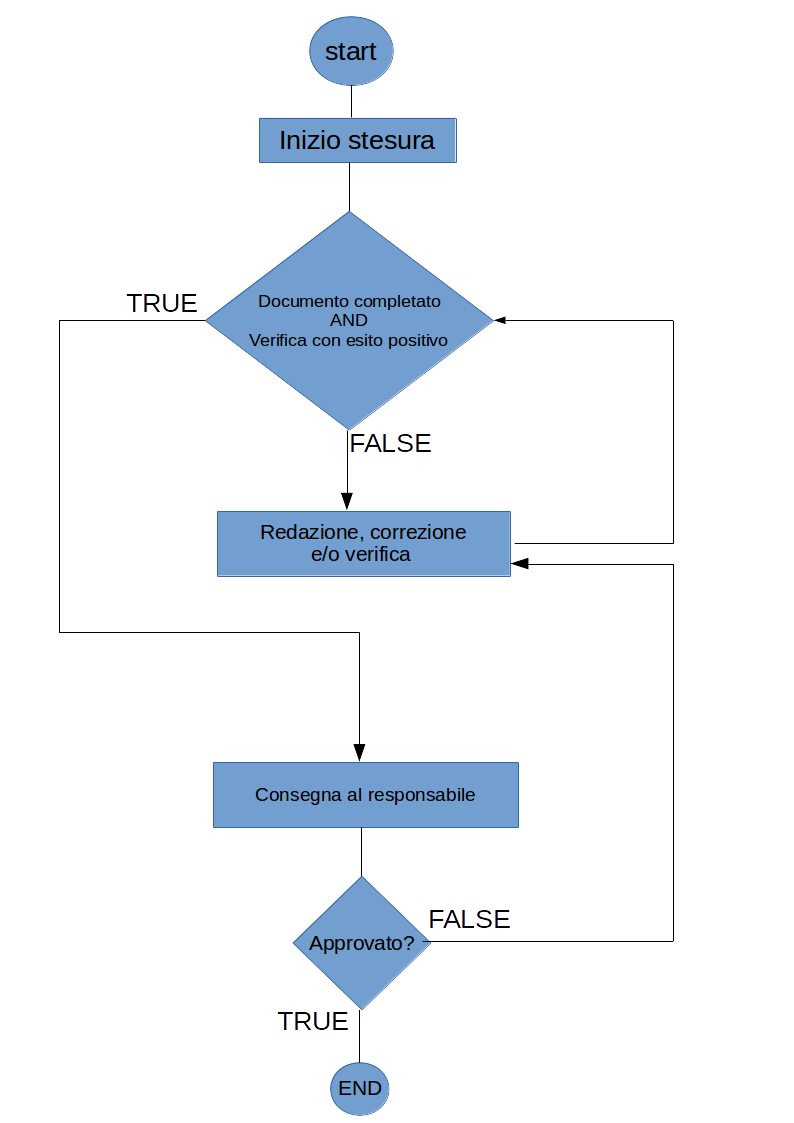
\includegraphics[scale=0.4]{img/flussoapprovazione.png}
\caption{Flow chart dell'approvazione di un documento}\label{sec:Figura2}
\end{figure}
\subsubsection{Template}
Per garantire omogeneità tra i documenti è stato creato un \gl{template} \LaTeX{}, dove sono state definite tutte le regole di formattazione da applicare al documento. Questo permette a tutti i componenti del gruppo di concentrarsi solo nella stesura del contenuto, senza doversi preoccupare dell'aspetto. 
\subsubsection{Struttura dei documenti}
 \paragraph{Frontespizio} 
La prima pagina di ogni documento dovrà contenere:
\begin{itemize}
	\item logo del gruppo;
	\item nome del \gl{progetto};
	\item nome del documento e la relativa versione;
	\item sommario;
	\item data di redazione;
	\item nome e cognome dei redattori del documento;
	\item nome e cognome dei verificatori del documento;
	\item nome e cognome del responsabile per l'approvazione del documento;
	\item uso del documento (interno o esterno);
	\item lista di distribuzione del documento.
\end{itemize}
 \paragraph{Diario delle modifiche}
 La seconda pagina dovrà contenere il diario delle modifiche di quel determinato documento.\\
 Il diario è costituito di una tabella ordinata in modo decrescente seconda la data di modifica e il numero di versione.\\
 Gli \gl{attributi} della tabella rappresentano:
 \begin{itemize}
 	\item numero di versione;
 	\item breve riepilogo delle modifiche apportate;
 	\item autore delle modifiche;
 	\item ruolo ricoperto dall'autore all'interno del \gl{progetto};
 	\item data di modifica.
 \end{itemize}
 \paragraph{Indice}
 In ogni documento è presente un indice delle sezioni, utile a fornire una visione macroscopica della struttura del documento. Sono previsti, se necessari, gli indici relativi alle tabelle e alle figure presenti nel documento in questo ordine.
 \paragraph{Intestazione e piè di pagina}
L'intestazione delle pagine di ogni documento deve contenere:
\begin{itemize}
	\item numero e titolo della sezione;
	\item nome del \gl{progetto}.
\end{itemize} 
Il piè di pagina contiene invece:
\begin{itemize}
	\item nome del documento con la relativa versione;
	\item nome del gruppo;
	\item pagina X di Y, dove X è la pagina corrente e Y è il numero di pagine totali del documento.
\end{itemize} 
\subsubsection{Versionamento}
Ciascun documento che verrà redatto dovrà essere versionato, per consentire un tracciamento chiaro della sua storia e delle sue modifiche.\\Verrà applicato il seguente formalismo:\\ \\ \centerline{vX.Y.Z}\\ \\dove:
\begin{itemize}
	\item \textbf{X}:
	\begin{itemize}
		\item inizia da 0;
		\item viene incrementato quando il \RESP{} di \gl{progetto} approva il documento.
	\end{itemize}
	\item \textbf{Y}:
	\begin{itemize}
		\item inizia da 0;
		\item viene incrementato dal \VER{} ad ogni \gl{verifica};
		\item quando viene modificato X, viene riportato a 0.
	\end{itemize}
	\item \textbf{Z}:
	\begin{itemize}
		\item inizia da 0;
		\item viene incrementato dal Redattore del documento dopo ogni modifica;
		\item quando viene modificato Y, viene riportato a 0.
	\end{itemize}
\end{itemize}
\subsubsection{Norme tipografiche}
In questa sezione vengono definite le norme ortografiche e tipografiche da rispettare nella stesura di ogni documento.
 \paragraph{Stile del testo} 
\begin{itemize}
	\item \textbf{Grassetto}: viene utilizzato per:
	\begin{itemize}
		\item titoli;
		\item elementi di un elenco puntato che riassumono il contenuto del relativo paragrafo.
	\end{itemize}
	\item \textbf{Corsivo}: viene utilizzato per:
	\begin{itemize}
		\item citazioni;
		\item abbreviazioni;
		\item parole inserite nel glossario;
		\item riferimenti ad altri documenti;
		\item nomi di società o aziende;
		\item ruoli dei membri del gruppo.
	\end{itemize}
	\item \textbf{Maiuscolo}: le parole scritte interamente in maiuscolo dovranno riferirsi soltanto ad acronimi.
	\item \textbf{Monospace}: le porzioni di testo scritte in monospace definiscono:
	\begin{itemize}
		\item frammenti di codice;
		\item comandi;
		\item URL.
	\end{itemize}
	\item \textbf{Glossario}: le parole che hanno un riferimento nel glossario sono in corsivo e hanno una 'g' a pedice.
\end{itemize}
 \paragraph{Elenchi puntati}
Tutti gli elenchi puntati sono caratterizzati graficamente da un pallino nel primo livello, da una trattino nel secondo e da un asterisco nel terzo (automatizzato grazie al \gl{template} \LaTeX{}{} creato). \\
Ogni elemento deve terminare con il punto e virgola, a meno che non sia l'ultimo dell'elenco, in questo caso la frase va terminata con il punto. Ogni punto inizia con la minuscola, tranne nel caso in cui necessiti di una spiegazione: allora
si utilizzerà la maiuscola.
 \paragraph{Formati comuni}
\begin{itemize}
	\item \textbf{Date}:\\ \\ \centerline{AAAA - MM - GG} \\ \\
	dove:
	\begin{itemize}
		\item AAAA: rappresenta l'anno utilizzando 4 cifre;
		\item MM: rappresenta il mese utilizzando 2 cifre;
		\item GG: rappresenta il giorno utilizzando 2 cifre.
	\end{itemize}
	\item \textbf{Orari}:\\ \\ \centerline{HH:MM} \\ \\dove:
	\begin{itemize}
		\item HH: rappresenta l'ora e può assumere valori da 0 a 23;
		\item MM: rappresenta i minuti e può assumere valori da 0 a 59.
	\end{itemize}
	\item \textbf{Nomi ricorrenti}:
	\begin{itemize}
		\item \textbf{Ruoli di \gl{progetto}}: ogni nome di un ruolo di \gl{progetto} deve essere scritto con la lettera iniziale maiuscola e con lo stile corsivo. Questo viene automatizzato utilizzando il comando "\textbackslash{CodiceRuolo}";
		\item \textbf{Nomi propri}: ogni nome deve essere espresso nella forma "Nome Cognome";
		\item \textbf{Nomi dei documenti}: ogni nome di documento viene scritto con lo stile corsivo, con l'iniziale di ogni parola maiuscola e con la versione corrente. Questo viene automatizzato richiamando il comando "\textbackslash{SiglaDocumentodoc}".
	\end{itemize}
\end{itemize}
 \paragraph{Sigle}
E' previsto l'utilizzo di queste sigle:
\begin{itemize}
	\item \textbf{AdR}: per \ARdoc;
	\item \textbf{PdP}: per \PPdoc;
	\item \textbf{NdP}: per \NPdoc;
	\item \textbf{SdF}: per \SFdoc;
	\item \textbf{PdQ}: per \PQdoc;
	\item \textbf{ST}: per \STdoc;
	\item \textbf{Gl}: per \Gldoc;
	\item \textbf{DP}: per \DPdoc.		
\end{itemize}
 
\subsubsection{Elementi grafici}
 \paragraph{Tabelle} 
 Le tabelle devono essere accompagnate da una didascalia e da un numero incrementale per
garantirne la tracciabilità.
 \paragraph{Immagini}
Ogni immagine deve essere centrata orizzontalmente. Inoltre deve
essere nettamente separata dai paragrafi che la seguono e la precedono, in modo da definire un netto distacco tra testo e grafica e migliorare conseguentemente la leggibilità. Essa dev'essere accompagnata da una didascalia analoga a quella descritta per le tabelle. Tutti i diagrammi
\gl{UML} vengono inseriti nel documento sotto forma di immagine.
\subsubsection{Classificazione dei documenti}
 \paragraph{Documenti informali}
 Tutti i documenti sono da ritenersi informali fino all'approvazione da parte del \RESP{} di \gl{progetto}, ed in quanto tali sono da considerarsi esclusivamente ad uso interno.
 \paragraph{Documenti formali}
 Un documento viene definito formale quando viene validato dal \RESP{} di \gl{progetto}. Solo i documenti formali possono essere distribuiti all'esterno del gruppo. Per arrivare a tale stato il
documento deve aver passato la \gl{verifica} e la \gl{validazione}.
 \paragraph{Glossario}
Il glossario nasce dall'esigenza di chiarire il significato di parole che possono risultare ambigue all'interno di determinati contesti. Saranno quindi presenti parole che:
\begin{itemize}
	\item trattano argomenti tecnici;
	\item possono creare delle ambiguità sul significato;
	\item rappresentano delle sigle.
\end{itemize}
La struttura deve avere queste caratteristiche:
\begin{itemize}
	\item le parole devono essere in ordine alfabetico;
	\item ogni termine deve essere seguito da una spiegazione chiara e concisa, che non generi alcun tipo di ambiguità.
\end{itemize}
 \paragraph{Verbali}
Questo documento ha lo scopo di riassumere in modo formale le discussioni effettuate e le decisioni prese durante le riunioni. I verbali, come le riunioni, sono classificati in: interni ed esterni. In
particolare i verbali esterni, essendo documenti ufficiali, devono essere redatti dal \RESP{} di Progetto.
Ogni verbale dovrà essere denominato nel seguente modo:\\ \\
\centerline{\textit{Verbale\textunderscore{TipoVerbale}\textunderscore{DataVerbale}}}
\\ \\
dove:
\begin{itemize}
	\item \textbf{TipoVerbale}: identifica se il verbale è riferito ad una riunione interna (I) o esterna (E);
	\item \textbf{DataVerbale}: identifica la data nella quale si è svolta la riunione relativa al verbale.
\end{itemize}
Nella parte introduttiva vengono specificate le seguenti informazioni:
\begin{itemize}
	\item luogo di incontro;
	\item data di incontro;
	\item orario di inizio;
	\item orario di fine;
	\item durata dell'incontro;
	\item oggetto dell'incontro;
	\item partecipanti;
	\item segretario;
	\item segnalazioni varie.
\end{itemize}
Tutte le decisioni prese durante la riunione vengono identificate univocamente utilizzando questo formato: \\ \\
\centerline{\textbf{DIX.Y} per i verbali interni}  \\ \\
\centerline{\textbf{DEX.Y} per i verbali esterni}  \\ \\
dove:
\begin{itemize}
	\item \textbf{X}: rappresenta il numero di verbale redatto in ordine cronologico (inizia da 1);
	\item \textbf{Y}: rappresenta il numero della decisione all'interno di un singolo verbale (inizia da 1).
\end{itemize}
Inoltre vengono tracciate le decisioni in sospeso che verranno chiarite in verbali successivi. Il formato identificativo è lo stesso delle decisioni definitive, dove nel codice la D viene sostituita dalla S.
\subsubsection{Strumenti}
\label{sec:Strumenti}
 \paragraph{\LaTeX{}}
La stesura dei documenti deve essere effettuata utilizzando il linguaggio di \gl{markup} \LaTeX{}. Le motivazioni di questa scelta sono dovute alle possibilità che \LaTeX{}{} offre:
\begin{itemize}
	\item creazione di documenti formali in modo rapido ed efficiente;
	\item possibilità di separare contenuto e formattazione, definendo l'aspetto delle pagine in un file
\gl{template} separato e condiviso da tutti i documenti;
	\item creazione e gestione automatica dell'indice del documento.
\end{itemize}
Inoltre è stato reso disponibile uno script PHP che per ogni documento \LaTeX{}{} marca tutte  le parole presenti nel \Gldoc{} secondo le regole decise nelle \NPdoc.
 \paragraph{\gl{Texmaker}}
Per la redazione del codice \LaTeX{}{} viene utilizzato l'editor \gl{Texmaker}. Questo
strumento oltre ad integrare un compilatore e visualizzatore \gl{PDF}, fornisce suggerimenti per il completamento dei comandi \LaTeX{}.
\begin{figure}[h]
\centering
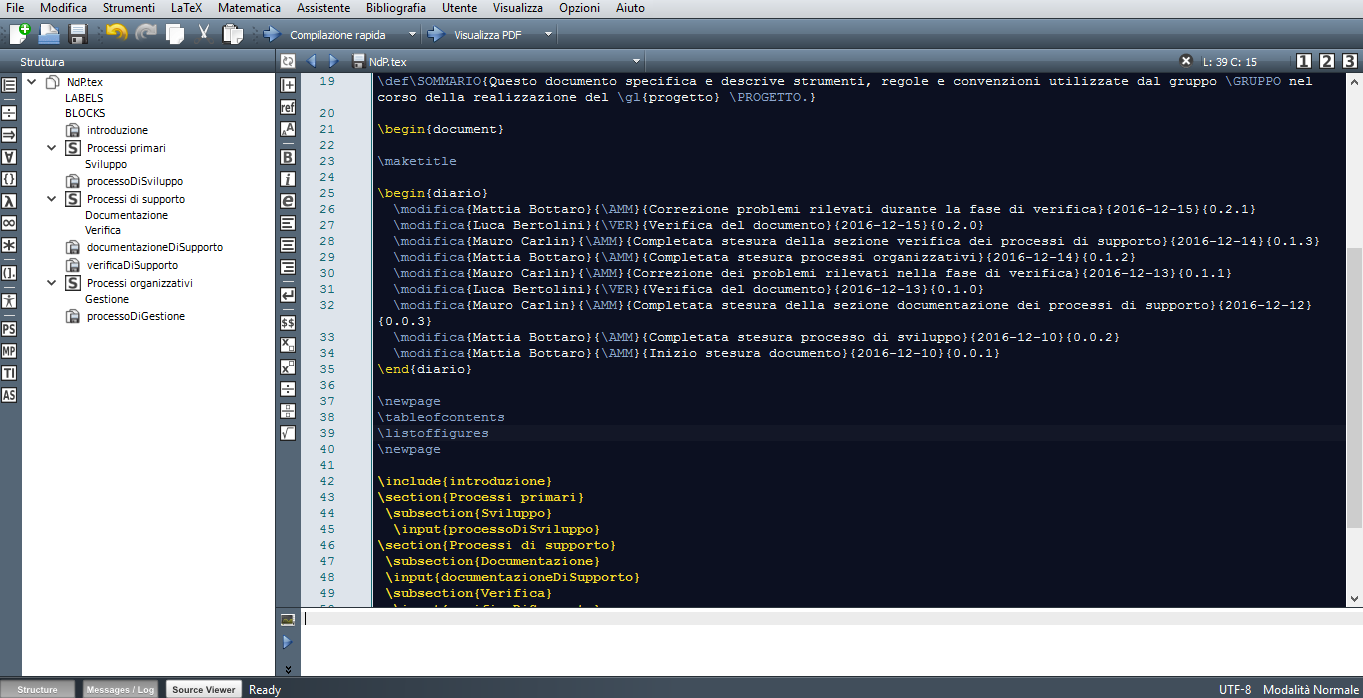
\includegraphics[scale=0.4]{img/texm.png}
\caption{Texmaker}\label{sec:Figura3}
\end{figure}
 \paragraph{Excel}
Per la creazione di grafici (istogrammi, diagrammi a torta, ecc.) viene utilizzato Excel di Microsoft Office, nella versione 2013 o successive.
 \subsection{Verifica}
  \subsubsection{Scopo del processo}
Si occupa di accertare che lo svolgimento del processo in esame non introduca errori nel \gl{prodotto}.
\subsubsection{Aspettative del processo}
Una corretta implementazione di tale processo permette di individuare:
\begin{itemize}
	\item una procedura di \gl{verifica};
	\item i criteri per la \gl{verifica} del \gl{prodotto}.
\end{itemize}
\subsubsection{Documenti}
Il \RESP{} ha il compito di avviare la fase di verifica, assegnando i task ai \VERP{}. Essi dovranno controllare che:
\begin{itemize}
	\item la sintassi sia corretta, facendo utilizzo degli strumenti automatici preposti e della tecnica walkthrough;
	\item i periodi non siano troppo lunghi, facendo utilizzo degli strumenti automatici preposti e della tecnica walkthrough;
	\item la struttura sia completa, non complicata e coerente con il contenuto del documento in esame.
\end{itemize}

\subsubsection{Diagrammi UML}
I \VERP{} devono controllare tutti i diagrammi UML prodotti, sia che
venga rispettato lo standard UML, sia che siano corretti semanticamente.
\paragraph{Diagrammi dei casi d'uso}
Per tutti i diagrammi d'uso, i \VERP{} dovranno controllare che:
\begin{itemize}
	\item rispettino lo standard UML;
	\item rappresentino ciò che dovrebbero modellare, facendo attenzione a inclusione, estensioni e generalizzazione;
	\item gli attori correlati siano corretti;
	\item non ci siano difetti grafici.
\end{itemize}
\paragraph{Diagrammi di sequenza}
Per tutti i diagrammi di sequenza, i \VERP{} dovranno controllare che:
\paragraph{Diagrammi di attività}
Per tutti i diagrammi di attività, i \VERP{} dovranno controllare che:
\paragraph{Diagramma dei package}
Per tutti i diagrammi dei package, i \VERP{} dovranno controllare che:
\subsubsection{Attività}
\paragraph{Analisi statica}
E' una tecnica di analisi del codice sorgente e della documentazione associata, prevalentemente
usata quando il \gl{sistema} non è ancora disponibile e durante tutto l'arco del suo sviluppo. Non
richiede l'esecuzione del \gl{prodotto} \gl{software} in alcuna sua parte. Può essere applicata tramite una
delle seguenti strategie:
\begin{itemize}
	\item \textbf{Walkthrough}: si legge l'intero documento (o codice) in cerca di tutte le possibili anomalie. E' una tecnica onerosa che richiede l'impegno di più persone e per questo deve essere utilizzata solo durante la prima parte del \gl{progetto}, dove non tutti i membri hanno piena padronanza e conoscenza delle \NPdoc e del \PQdoc;
	\item \textbf{Inspection}: questa tecnica dev'essere applicata quando si ha idea della
	problematica che si sta cercando; consiste in una lettura mirata del
	documento (o del codice), sulla base di una lista degli errori precedentemente
	stilata.
\end{itemize}
\paragraph{Analisi dinamica}
L'attività di analisi dinamica è una tecnica di \gl{verifica} applicabile solamente al \gl{software}. Tale tecnica può essere utilizzata per analizzare l'intero \gl{software} o una
porzione limitata dello stesso. L'attività consiste nell'esecuzione di test automatici realizzati
dal team. Le verifiche devono essere effettuate su un insieme finito di casi, con valori di
ingresso, uno stato iniziale e un esito decidibile. Tutti i test producono risultati automatici
che inviano notifiche sulla tipologia di problema individuato. Ogni test è ripetibile, ossia
applicabile durante l'intero \gl{ciclo di vita} del \gl{software}.

\subsubsection{Procedure}
\paragraph{Issue tracking}
L'\gl{issue} tracking è un'attività di supporto per la figura dei \VERP, ai quali permette di tenere traccia, e contemporaneamente segnalare al \RESP, la presenza di potenziali errori in un documento o nel codice sorgente.
 \subparagraph{Gestione delle \gl{issue}}
Qualora un \VER{} dovesse riscontrare delle anomalie, la procedura per la segnalazione e gestione del \gl{ticketing} di una \gl{issue} è la seguente:
\begin{enumerate}
	\item il \VER{} dovrà aprire una nuova \gl{issue} assegnandole una label che si riferisca al problema trovato;
	\item il \RESP{} di \gl{progetto} dovrà valutare la \gl{issue}; se la ritiene appropriata assegnerà ai redattori del documento (o ai \PRP) il compito di risolvere la \gl{issue};
	\item una volta risolta, e verificata, la \gl{issue} dovrà essere marcata come conclusa da parte del \RESP{} o del \VER;
\end{enumerate}
\subsubsection{Strumenti}
\paragraph{Strumenti per l'issue tracking}
Lo strumento utilizzato per l'\gl{issue} tracking è il servizio Issues messo a disposizione da \gl{GitHub}.
\paragraph{Verifica ortografica}
Viene utilizzata la \gl{verifica} in tempo reale dell'ortografia, integrata in TexMaker. Essa marca,
sottolineando in rosso, le parole errate secondo la lingua italiana.
\paragraph{Indice di Gulpease}
Affinché un documento possa superare la fase di approvazione, è necessario che soddisfi il test di leggibilità con un indice Gulpease superiore a 40 punti.
 \subsection{Validazione}
 \subsubsection{Scopo}
 Lo scopo di questo processo è verificare il prodotto ottenuto sia coerente rispetto gli obiettivi prefissati.
 \subsubsection{Aspettative}
 Le aspettative di questo processo sono che:
 \begin{itemize}
 	\item il prodotto finale rispetti i parametri di qualità imposti;
 	\item il prodotto finale sia conforme rispetto le aspettative;
 	\item il prodotto finale sia corretto.
 \end{itemize}
 \subsubsection{Descrizione}
 Le responsabilità sono così distribuite:
 \begin{itemize}
 	\item i \VERP{} hanno il compito di eseguire i test, tracciandone i risultati;
 	\item il \RESP{} revisiona i risultati dei test, decidendo se ritenerli accettabili o meno. Inoltre, si assume la responsabilità con il committente della conformità del prodotto finale rispetto le aspettative.
 \end{itemize}
 \subsubsection{Procedure}
 La procedura di validazione è composta dai seguenti punti:
 \begin{itemize}
 	\item i \VERP{} effettuano test manuali sul prodotto finale, tracciandone i risultati;
 	\item il \RESP{} esamina i risultati e decide se ritenerli buoni o se ripetere i test;
 	\item se accettati, il \RESP{} dovrà consegnare i risultati al proponente.
 \end{itemize}
 \newpage

\subsection{Qualità}
\subsubsection{Notazione}
\paragraph{Metriche}
Per garantire la qualità del lavoro del team gli \AMMP{} hanno definito delle metriche, riportandole
nel \PQdoc, che devono rispettare la seguente notazione:\\ \\
\centerline{\textbf{M\textbraceleft{}X\textbraceright{}\textbraceleft{}Y\textbraceright{}\textbraceleft{}Z\textbraceright{}}} \\ \\
dove:
\begin{itemize}
	\item \textbf{X} indica se la metrica si riferisce a prodotti o processi e può assumere
	i valori:
	\begin{itemize}
		\item \textbf{PC} per indicare i processi;
		\item \textbf{PD} per indicare i prodotti.
	\end{itemize}
	\item \textbf{Y} presente solo se la metrica è riferita ai prodotti, indica se il termine \gl{prodotto} si riferisce a documenti o al software e può assumere i seguenti valori:
	\begin{itemize}
		\item \textbf{D} per indicare i documenti;
		\item \textbf{S} per indicare il software;
	\end{itemize}
	\item \textbf{Z} indica il codice univoco della metrica (numero intero incrementale a partire da 1).
\end{itemize}
\paragraph{Obiettivi}
Per garantire la qualità del lavoro del team, gli \AMMP{} hanno definito degli obiettivi di qualità,
riportandoli nel \PQdoc, che devono rispettare la seguente notazione:\\ \\
\centerline{\textbf{O\textbraceleft{}X\textbraceright{}\textbraceleft{}Y\textbraceright{}\textbraceleft{}Z\textbraceright{}}} \\ \\
dove:
\begin{itemize}
	\item \textbf{X} indica se l'obiettivo si riferisce a prodotti o processi e può assumere i valori:
	\begin{itemize}
		\item \textbf{PC} per indicare i processi;
		\item \textbf{PD} per indicare i prodotti.
	\end{itemize}
	\item \textbf{Y} presente solo se l'obiettivo è riferito ai prodotti, indica se il termine \gl{prodotto} si riferisce a documenti o al software e può assumere i seguenti valori:
	\begin{itemize}
		\item \textbf{D} per indicare i documenti;
		\item \textbf{S} per indicare il software;
	\end{itemize}
	\item \textbf{Z} indica il codice univoco dell'obiettivo (numero intero incrementale a partire da 1).
\end{itemize}
\subsubsection{Definizione metriche}
Di seguito sono definite le metriche utilizzate nel documento \PQdocRP{}. Ad ogni metrica è stata assegnato un codice identificativo per facilitare il tracciamento.
\paragraph{Qualità di processo}
\subparagraph{Percentuale di accessi avvenuti correttamente a PragmaDB - MPC1}
Indica il numero  di accessi avvenuti correttamente espresso in percentuale.\\
\begin{equation*} 
\text{Percentuale accessi} = \frac{\text{Accessi avvenuti}}{\text{Richieste d'accesso}} * 100
\end{equation*}
\subparagraph{Schedule Variance - MPC2}
Indica se si è in linea, in anticipo o in ritardo rispetto ai tempi pianificati.\\
\begin{equation*}
\text{Schedule Variance = TP - TR} 
\end{equation*}
\begin{itemize}
	\item \textbf{TP} è il tempo pianificato per terminare un attività;
	\item \textbf{TR} è il tempo reale che è stato impiegato.
\end{itemize}		
\subparagraph{Cost Variance in percentuale - MPC3}
Indica se alla data corrente i costi corrispondono alla pianificazione, espressi in percentuale.
\begin{equation*}
\text{Cost Variance} = \frac{CP - CR}{CP} * 100
\end{equation*}
\begin{itemize}
	\item \textbf{CP} sono i costi pianificati per la data corrente;
	\item \textbf{CR} sono i costi reali sostenuti.
\end{itemize}
\subparagraph{Indice dei rischi non preventivati - MPC4}
É un indice che viene incrementato ogniqualvolta si manifesta un rischio non individuato nell'attività di analisi dei rischi.
\subparagraph{Numero di requisiti obbligatori soddisfatti - MPC5}
Indica la percentuale di requisiti obbligatori soddisfatti del prodotto.
\begin{equation*}
Numero requisiti = \frac{\text{requisiti obbligatori soddisfatti}}{\text{requisiti obbligatori totali}} * 100
\end{equation*}
\subparagraph{Numero di requisiti desiderabili soddisfatti - MPC6}
Indica la percentuale di requisiti desiderabili soddisfatti del prodotto.
\begin{equation*}
\text{Numero requisiti} = \frac{\text{requisiti desiderabili soddisfatti}}{\text{requisiti desiderabili totali}} * 100
\end{equation*}
\subparagraph{Numero di requisiti opzionali soddisfatti - MPC7}
Indica la percentuale di requisiti opzionali soddisfatti del prodotto.
\begin{equation*}
\text{Numero requisiti} = \frac{\text{requisiti opzionali soddisfatti}}{\text{requisiti opzionalii totali}} * 100
\end{equation*}
\subparagraph{SF-IN - MPC8}
Indice numerico che incrementa nel momento in cui viene individuato un modulo che, durante la sua esecuzione, chiama il modulo in oggetto.
\subparagraph{SF-OUT - MPC9}
Indice numerico che incrementa nel momento in cui viene individuato un modulo utilizzato dal modulo in oggetto durante la sua esecuzione.
\subparagraph{Numero di metodi per classe - MPC10}
Indica il numero di metodi definiti in ogni classe.
\subparagraph{Numero di parametri per metodo - MPC11}
Indica il numero di parametri definiti in ogni metodo.
\subparagraph{Indice di complessità ciclomatica - MPC12}
Dato un grafo non fortemente connesso che rappresenta una sezione di codice del software, indica il numero di cammini linearmente indipendenti.
\begin{equation*}
\text{Complessità ciclomatica} = E - N + 2P
\end{equation*}
\begin{itemize}
	\item \textbf{E} è il numero di archi del grafo;
	\item \textbf{N} è il numero di nodi del grafo;
	\item \textbf{P} è il numero di componenti connesse.
\end{itemize}
\subparagraph{Numero di livelli di annidamento - MPC13}
Indica il numero di procedure e funzioni annidate, ovvero richiamate all'interno di altre procedure o funzioni.
\subparagraph{Percentuale di linee di commento per linee di codice - MPC14}
Indica la percentuale di linee di commento rispetto alle linee di codice.
\begin{equation*}
\text{Percentuale linee di commento} = \frac{\text{Linee di commento}}{\text{Linee totali di codice}} * 100
\end{equation*}
\subparagraph{Indice di manutenibilità - MPC15}
Indica quanto sarà semplice mantenere il codice prodotto.
\begin{equation*}
\text{Manutenibilità} =\frac{(171 - 5,2 * \ln(V) - 0.23 * (\text{Complessita ciclomatica}) - 16.2 * \ln(\text{Linee di codice})*100)}{171}
\end{equation*}
dove 
\begin{equation*}
\begin{align*}
\text{V} = & (\text{Numero totale di operatori} + \text{Numero totale di operandi})* \\ 
& \log_2 (\text{Numero di operatori distinti}+\text{Numero di operandi distinti})
\end{align*}
\end{equation*}

\subparagraph{Percentuale di componenti integrate nel sistema - MPC16}
Indica la percentuale di componenti attualmente implementate e correttamente integrate nel sistema.
\begin{equation*}
\text{Componenti integrate} = \frac{\text{Numero componenti integrate}}{\text{Numero componenti totali progettate}} * 100
\end{equation*}
\subparagraph{Percentuale di test di unità eseguiti - MPC17}
Indica la percentuale di test di unità eseguiti.
\begin{equation*}
\text{Test di unità eseguiti} = \frac{\text{Numero test di unita eseguiti}}{\text{Numero test di unita pianificati}} * 100
\end{equation*}
\subparagraph{Percentuale di test di integrazione eseguiti - MPC18}
Indica la percentuale di test di integrazione eseguiti.
\begin{equation*}
\text{Test di integrazione eseguiti} = \frac{\text{Numero test di integrazione eseguiti}}{\text{Numero test di integrazione pianificati}} * 100
\end{equation*}
\subparagraph{Percentuale di test di sistema eseguiti - MPC19}
Indica la percentuale di test di sistema eseguiti.
\begin{equation*}
\text{Test di sistema eseguiti} = \frac{\text{Numero test di sistema eseguiti}}{\text{Numero test di sistema pianificati}} * 100
\end{equation*}
\subparagraph{Percentuale di test di validazione eseguiti - MPC20}
Indica la percentuale di test di validazione eseguiti.
\begin{equation*}
\text{Test di validazione eseguiti} = \frac{\text{Numero test di validazione eseguiti}}{\text{Numero test di validazione pianificati}} * 100
\end{equation*}
\subparagraph{Percentuale dei test superati - MPC21}
Indica la percentuale di test superati.
\begin{equation*}
\text{Test superati} = \frac{\text{Numero test superati}}{\text{Numero test eseguiti}} * 100
\end{equation*}
\subparagraph{Percentuale di rami decisionali percorsi - MPC22}
Indica la percentuale di rami decisionali percorsi dai test utilizzati.
\begin{equation*}
\text{Rami decisionali percorsi} = \frac{\text{Numero rami decisionali percorsi}}{\text{Numero rami decisionali totali}} * 100
\end{equation*}
\subparagraph{Numero di funzioni chiamate nei test - MPC23}
Indica il numero di funzioni chiamate nei test utilizzati.
\begin{equation*}
\text{Numero di funzioni chiamate} = \frac{\text{Funzioni chiamate}}{\text{Numero di funzioni totali}} * 100
\end{equation*}

\subparagraph{Numero di istruzioni nei test - MPC24}
Indica il numero di istruzioni eseguite nei test utilizzati.

\begin{equation*}
\text{Numero di istruzioni} = \frac{\text{Istruzioni eseguite}}{\text{Istruzioni totali}} * 100
\end{equation*}


\paragraph{Qualità di prodotto}
\subparagraph{Indice Gulpease - MPDD1}
Permette di calcolare i livello di leggibilità e comprensibilià del documento.

\begin{equation*}\textit{Indice Gulpease} = 89 + \frac{300 * \textit{A} + 10 * B}{C}\end{equation*} \\
\begin{itemize}
	\item \textbf{A} è il numero totale di frasi;
	\item \textbf{B} è il numero totale di lettere
	\item \textbf{C} è il numero totale di parole;
\end{itemize}
\subparagraph{Completezza dell’implementazione funzionale - MPDS1}
Permette di calcolare i livello di leggibilità e comprensibilià del documento.

\begin{equation*}
C=(1-\frac{FM}{FI})\cdot 100
\end{equation*}
\begin{itemize}
	\item \textbf{FM} è il numero di funzionalità mancanti nell'implementazione;
	\item \textbf{FI} è il numero di funzionalità individuate nell'attività di analisi;
\end{itemize}
\subparagraph{Percentuale di risultati concordi alle attese - MPDS2}
Calcola quanti risultati sono concordi alle attese.

\begin{equation*} RC = (1-\frac{N_{RD}}{N_{TE}}) \cdot 100 \end{equation*}
\begin{itemize}
	\item \textbf{RD} è il numero di test che producono risultati discordanti rispetto alle attese;
	\item \textbf{TE}  è il numero di test-case eseguiti;
\end{itemize}
\subparagraph{Percentuale di operazioni illegali non bloccate - MPDS3}
Calcola quante operazioni illegali non sono state bloccate.

\begin{equation*}I=\frac{N_{IE}}{N_{II}} \cdot 100\end{equation*}
\begin{itemize}
	\item \textbf{IE} è il numero di operazioni illegali effettuabili dai test;
	\item \textbf{II} è il numero di operazioni illegali individuate;
\end{itemize}
\subparagraph{Percentuale failure su test-case - MPDS4}
Calcola la percentuale di operazioni di testing che si sono concluse in failure.

\begin{equation*}F=\frac{N_{FR}}{N_{TE}} \cdot 100 \end{equation*}
\begin{itemize}
	\item \textbf{FR} è il numero di failure rilevati durante l'attività di testing;
	\item \textbf{TE} è il numero di test-case eseguiti;
\end{itemize}
\subparagraph{Numero di failure evitati - MPDS5}
Calcola la percentuale di funzionalità in grado di gestire correttamente i fault che potrebbero verificarsi.

\begin{equation*}B=\frac{N_{FE}}{N_{ON}} \cdot 100 \end{equation*}
\begin{itemize}
	\item \textbf{FE} è il numero di failure evitati durante i test effettuati;
	\item \textbf{ON} è il numero di test-case eseguiti che prevedono l'esecuzione di operazioni non corrette, causa di possibili failure;
\end{itemize}
\subparagraph{Percentuale delle funzionalità comprese  - MPDS6}
Calcola la percentuale di operazioni comprese in modo immediato dall'utente, senza la consultazione del manuale.

\begin{equation*}C=\frac{N_{FC}}{N_{FO}} \cdot 100\end{equation*}
\begin{itemize}
	\item \textbf{FC} è il numero di funzionalità comprese in modo immediato dall'utente durante l'attività di testing del prodotto;
	\item \textbf{FO} è il numero di funzionalità offerte dal sistema;
\end{itemize}
\subparagraph{Percentuale di funzionalità conformi alle aspettative - MPDS7}
Calcola la percentuale di funzionalità offerte all'utente che rispettano le sue aspettative riguardo al comportamento del software.

\begin{equation*}C=(1-\frac{N_{MFI}}{N_{MFO}}) \cdot 100\end{equation*}
\begin{itemize}
	\item \textbf{MFI} è il numero di messaggi e funzionalità che non rispettano le aspettative dell'utente;
	\item \textbf{MFO} è il numero di messaggi e funzionalità offerti dal sistema;
\end{itemize}
\subparagraph{Tempo medio di risposta - MPDS8}
Calcola il periodo temporale medio trascorso tra la richiesta al software di una determinata funzionalità e la risposta all’utente.

\begin{equation*}T_{RISP} = \frac{\sum_{i=1}^{n} T_{i}}{n}\end{equation*}
\begin{itemize}
	\item \textbf{$T_{RISP}$} espresso in \textit{secondi};
	\item \textbf{$T_{i}$} è il tempo intercorso fra la richiesta $i$ di una funzionalità ed il completamento delle operazioni necessarie a restituire un risultato a tale richiesta;
\end{itemize}
\subparagraph{Percentuale di failure con cause individuate - MPDS9}
Calcola la percentuale di failure di cui sono state individuate le cause.

\begin{equation*}I=\frac{N_{FI}}{N_{FR}} \cdot 100 \end{equation*}
\begin{itemize}
	\item \textbf{FI}  è il numero di failure delle quali sono state individuate le cause;
	\item \textbf{FR} è il numero di failure rilevate;
\end{itemize}
\subparagraph{percentuale di failure introdotte con modifiche - MPDS10}
Calcola la percentuale di modifiche effettuate in risposta a failure che hanno portato all'introduzione di nuove failure in altre componenti del sistema.

\begin{equation*}I=\frac{N_{FRF}}{N_{FR}} \cdot 100 \end{equation*}
\begin{itemize}
	\item \textbf{FRF}  è il numero di failure risolte con l'introduzione di nuove failure;
	\item \textbf{FR} è il numero di failure risolte;
\end{itemize}

\subsubsection{Procedure}
\paragraph{Calcolo dell'indice di Gulpease}
Affinché un documento possa superare la fase di approvazione, è necessario che soddisfi il test di leggibilità con un indice Gulpease superiore a 40 punti. Per valutare questa metrica di qualità, è necessario seguire la seguente procedura:
\begin{itemize}
	\item dirigersi da terminale in \GulScript{};
	\item dare il comando \file{php gulpease.php};
	\item visualizzare il risultato sul terminale.
\end{itemize}
\paragraph{Controllo ortografico}
Per verificare la correttezza ortografica è necessario seguire la seguente procedura:
\begin{itemize}
	\item aprire Texmaker;
	\item aprire il documento interessato nel formato .tex;
	\item dal menù a tendina "Modifica", selezionare la voce "verifica ortografia".
\end{itemize}
Per rendere ciò possibile, è necessario installare il pacchetto relativo dizionario italiano per Texmaker.
\paragraph{Resoconto stato metriche}
Per visualizzare il resoconto corrente dello stato di ciò che le metriche indicano, è necessario seguire la seguente procedura:
\begin{itemize}
	\item effettuare l'accesso in PragmaDB;
	\item selezionare la voce "Metriche".
\end{itemize}
\paragraph{Resoconto stato test di unità}
Per visualizzare il resoconto corrente dello stato dei test di unità è necessario seguire la seguente procedura:
\begin{itemize}
	\item entrare nella cartella \texttt{/responsoTest};
	\item aprire il file corrispondente al test eseguito, identificato con data e ora dell'esecuzione.
\end{itemize}
\paragraph{Resoconto stato build}
Per visualizzare il resoconto corrente dello stato di una delle build eseguite, è necessario seguire la seguente procedura:
\begin{itemize}
	\item entrare nella cartella \texttt{/statoBuild};
	\item aprire il file corrispondente al numero della build sulla quale si vogliono informazioni.
\end{itemize}

\subsubsection{Strumenti}
\paragraph{Script per il calcolo dell'indice di Gulpease}
In \GulScript{} si trova lo script che calcola l'indice di Gulpease per ogni documento.
\paragraph{Controllo ortografico}
Per il controllo ortografico dei documenti si farà utilizzo dello strumento integrato in Texmaker.\\
Per poterlo utilizzare, è necessario disporre del pacchetto per il dizionario italiano.
\paragraph{Integrazione continua - Jenkins}
Jenkins è uno strumento open source di continuous integration, scritto in linguaggio Java che fornisce dei servizi di integrazione continua per lo sviluppo del software. Viene eseguito lato server all'interno di un server web che supporta la tecnologia Servlet e quindi può essere utilizzato da remoto all'interno di un Web browser.\\
Questo strumento permetterà al gruppo di automatizzare i test di unità, che verranno eseguiti ad ogni push eseguita da un programmatore, ed il processo di build e deployment del prodotto.
\subparagraph{Codifica ed esecuzione test di unità - Mocha}
Mocha è un framework che permette di creare ed eseguire test sia per Node.js che per il browser web.
\subparagraph{Calcolo della copertura dei test - Istanbul}
Istanbul è uno strumento che calcola la copertura dei test rispetto a statement, righe, funzioni e branch di un determinato progetto.


\paragraph{Requisiti obbligatori soddisfatti}
Lo strumento scelto per il calcolo del valore di questa metrica è PragmaDB, il quale permette di tracciare i requisiti ed associarli su use case e fonti.
\paragraph{Requisiti accettati soddisfatti}
Lo strumento scelto per il calcolo del valore di questa metrica è PragmaDB, il quale permette di tracciare i requisiti ed associarli su use case e fonti.
\paragraph{Requisiti non accettati soddisfatti}
Lo strumento scelto per il calcolo del valore di questa metrica è PragmaDB, il quale permette di tracciare i requisiti ed associarli su use case e fonti.
\paragraph{Requisiti obbligatori soddisfatti}
Lo strumento scelto per il calcolo del valore di questa metrica è PragmaDB, il quale permette di tracciare i requisiti ed associarli su use case e fonti.
\paragraph{Structural Fan-In}
Lo strumento scelto per il calcolo del valore di questa metrica è PragmaDB, il quale permette di tracciare quanti moduli durante la loro esecuzione utilizzano un determinato modulo.
\paragraph{Structural Fan-Out}
Lo strumento scelto per il calcolo del valore di questa metrica è PragmaDB, il quale permette di tracciare quanti moduli vengono utilizzate durante l'esecuzione di un determinato modulo.
\paragraph{Metodi per classe}
Lo strumento scelto per il calcolo del valore di questa metrica è PragmaDB, il quale permette di tracciare il numero di metodi per ogni classe.
\paragraph{Parametri per metodo}
Lo strumento scelto per il calcolo del valore di questa metrica è PragmaDB, il quale permette di tracciare il numero di parametri per ogni metodo.
\paragraph{Componenti integrate}
Lo strumento scelto per il calcolo del valore di questa metrica è PragmaDB, il quale permette di tracciare le componenti che sono attualmente implementate e integrate nel sistema.
\paragraph{Test di unità eseguiti}
Lo strumento scelto per il calcolo del valore di questa metrica è PragmaDB, il quale permette di tracciare i test di unità eseguiti.
\paragraph{Test di integrazione eseguiti}
Lo strumento scelto per il calcolo del valore di questa metrica è PragmaDB, il quale permette di tracciare i test di integrazione eseguiti.
\paragraph{Test di sistema eseguiti}
Lo strumento scelto per il calcolo del valore di questa metrica è PragmaDB, il quale permette di tracciare i test di sistema eseguiti.
\paragraph{Test di validazione eseguiti}
Lo strumento scelto per il calcolo del valore di questa metrica è PragmaDB, il quale permette di tracciare i test di validazione eseguiti.
\paragraph{Test superati}
Lo strumento scelto per il calcolo del valore di questa metrica è PragmaDB, il quale permette di tracciare i test superati.
\paragraph{Completezza implementazione funzionale}
Lo strumento scelto per il calcolo del valore di questa metrica è PragmaDB, il quale permette di tracciare il numero di requisiti funzionali implementati.
\paragraph{Densità di failure}
Lo strumento scelto per il calcolo del valore di questa metrica è PragmaDB, il quale permette di tracciare le operazioni di testing che sono concluse in failure.


\newpage
\section{Processi organizzativi}
 \subsection{Gestione}
  \subsubsection{Scopo}
Lo scopo del processo è produrre il \PPdoc , al fine di pianificare e gestire i ruoli che i membri dovranno assumere.
\subsubsection{Aspettative}
Le aspettative del processo sono:
 \begin{itemize}
  \item produrre il \PPdoc ;
  \item definire i ruoli dei membri del gruppo;
  \item definire il piano per l'esecuzione dei compiti programmati.
 \end{itemize}
\subsubsection{Descrizione}
 
\subsubsection{Ruoli di progetto}
 In ogni momento temporale ogni membro deve ricoprire almeno un ruolo e, durante tutta la durata del \gl{progetto}, ricoprire tutti i ruoli almeno una volta. Per ogni membro, le ore di lavoro devono essere il più possibile equamente distribuite. L'assegnazione e la rotazione dei ruoli sono pianificate nel \PPdocRR.
 \paragraph{Responsabile}
 Il \RESP{} è il rappresentante e il punto di riferimento del gruppo, nonché colui che si assume le responsabilità delle scelte del gruppo.
 Le responsabilità assunte sono:
 \begin{itemize}
  \item pianificazione, coordinamento e controllo delle attività;
  \item gestione delle risorse;
  \item analisi e gestione dei rischi;
  \item approvazione dei documenti;
  \item approvazione dell'offerta economica;
  \item convocazione delle riunioni interne;
  \item relazioni esterne;
  \item assegnazione delle attività a persone.
\end{itemize}
Per questi motivi ha il compito di:
\begin{itemize}
	\item assicurarsi che le attività di verifica e validazione siano svolte seguendo le \NPdoc;
	\item garantire il rispetto dei ruoli e dei compiti assegnati nel \PPdoc.
\end{itemize}
 \paragraph{Amministratore}
 L'\AMM{} è responsabile dell'efficienza dell'ambiente di lavoro, in particolare si occupa di:
 \begin{itemize}
  \item studiare e fornire strumenti che migliorano l'ambiente di lavoro, automatizzando il lavoro ove possibile;
  \item gestire archiviazione, versionamento e configurazione dei documenti e del \gl{software};
  \item garantire la qualità del \gl{prodotto}, fornendo procedure e strumenti di monitoraggio e segnalazione;
  \item eliminare le difficoltà sulla gestione di processi e risorse.
 \end{itemize}
 L'\AMM{} non compie scelte gestionali, ma tecnologiche concordate con il \RESP.
 \paragraph{Analista}
 L'\AN{} deve identificare e comprendere il dominio del problema. \\
 In particolare si occupa di:
 \begin{itemize}
  \item mappare le richieste del cliente in specifiche per il \gl{prodotto};
  \item catalogare e spiegare specifiche comprensibili nell'\ARdoc{} e nello \SFdoc{};
  \item classificare i requisiti;
  \item stendere i diagrammi dei casi d'uso;
  \item assegnare i requisiti a parti distinte del sistema;
  \item assicurarsi che i requisiti trovati siano conformi alle richieste del proponente;
  \item definire test di sistema e di accettazione al fine di verificare i requisiti.
\end{itemize}
L'\AN{} non si occupa di trovare una soluzione al problema, ma lo definisce redigendo lo \textit{"Studio di Fattibilità"} e l'\textit{"Analisi dei Requisiti"}. 

 \paragraph{Progettista}
 Il \PJ{} ha forti competenze sullo \gl{stack} tecnologico usato. \\
 In particolare deve: 
 \begin{itemize}
  \item indicare le tecnologie più adatte allo sviluppo del \gl{progetto};
  \item descrivere il funzionamento del \gl{sistema} progettandone l'architettura;
  \item produrre una soluzione fattibile in termini di risorse.
 \end{itemize}
Il \PJ{} redige i documenti di \textit{"Specifica Tecnica"}, \textit{"Definizione di prodotto"} e si occupa delle sezioni del \textit{"Piano di Qualifica"} relative alle metriche di verifica della programmazione.
\newpage
\paragraph{Programmatore}
 Il \PR{} si occupa della codifica, in particolare:
 \begin{itemize}
  \item implementa le soluzioni indicate dal \PJ ;
  \item scrive codice documentato, versionato e mantenibile nel rispetto delle \NPdoc ;
  \item realizza e fornisce gli strumenti per verificare e validare il \gl{prodotto}.
 \end{itemize}
 \paragraph{Verificatore}
 Il \VER , disponendo di una profonda conoscenza delle \NPdoc , si occupa delle attività di \gl{verifica}. \\
 In particolare deve: 
 \begin{itemize}
  \item controllare il rispetto delle \NPdoc durante ogni attività del \gl{progetto}.
 \end{itemize}
 \paragraph{Rotazione dei ruoli}
 Ogni membro del gruppo dovrà ricoprire ciascuno dei ruoli del progetto. La pianificazione dovrà essere redatta prestando attenzione a quanto segue:
 \begin{itemize}
 	\item ogni membro del gruppo non dovrà mai ricoprire un ruolo che preveda la verifica dell'operato svolto da lui in precedenza poiché questo potrebbe portare ad un conflitto di interesse;
 	\item bisogna tener conto dei possibili impegni o interessi dei singoli membri del gruppo;
 	\item ciascun membro dovrà assicurare l'esclusivo svolgimento del ruolo a lui assegnato.
 \end{itemize}  
\subsubsection{Comunicazioni}
 \paragraph{Interne}
 È stato creato un gruppo Telegram, accessibile solo ai membri del team, per effettuare le comunicazioni interne. In caso siano necessaria maggiore interazione, si farà utilizzo di \gl{Google Hangouts}. 
 \paragraph{Esterne}
 È stata creata un'apposita cartella di posta elettronica per mantenere i contatti con il \gl{proponente}, il committente ed altre eventuali figure esterne.\\
  Inoltre, su richiesta dell'azienda proponente \PROPONENTE, è stato creato un apposito dominio Slack per permettere una veloce interazione tra i gruppi fornitori e l'azienda. Il dominio è zero12university. \\
 La gestione della casella di posta elettronica e di Slack è compito del \RESP. \\
 L'indirizzo e-mail è il seguente: \EMAIL.
 \paragraph{Email}
 Le mail devono essere scritte nella maniera più chiara e corretta possibile, in particolare ognuna di esse deve essere composta di:
 \begin{itemize}
 	\item destinatario;
 	\item oggetto, che deve essere breve e diretto;
	\item contenuto, che deve essere chiaro ed esaustivo;
	\item firma del responsabile.
 \end{itemize}
 Nel caso si vogliano scambiare dei documenti, si deve a evitare l'invio di allegati tramite email e preferire l'utilizzo di un apposito sito di scambi, quale ad esempio Google Drive.
\subsubsection{Incontri}
 \paragraph{Interni}
 Ogni membro del team può proporre un incontro interno tramite il \gl{bot} Telegram \gl{VotePoll}, specificando i motivi e l'oggetto dell'incontro. 
 Sarà poi compito del \RESP{} decidere se effettuare l'incontro o meno.\\
  La verbalizzazione degli incontri interni è compito di uno tra gli \AMMP.
 \paragraph{Esterni} 
 Ogni membro del team può proporre un incontro esterno tramite il \gl{Bot} Telegram "\gl{VotePoll}", specificando i motivi e l'oggetto dell'incontro. 
Se il \RESP{} decide che l'incontro può essere organizzato dovrà accordarsi con la figura esterna, e comunicare gli estremi della riunione ai membri del team.\\
 La verbalizzazione degli incontri esterni è compito del \RESP.
 \paragraph{Gestione}
 All’inizio di ogni riunione interna il \RESP{} nomina l'amministratore che ha il compito di tracciare gli aspetti più importanti della riunione, con lo scopo di esporli poi nel relativo verbale. Questo verbale verrà archiviato nel repository del gruppo, in modo da permetterne la consultazione. Se invece la riunione è esterna, questo compito è delegato al \RESP{}.
 Durante le riunioni i partecipanti devono tenere un comportamento che favorisca la discussione all’interno del gruppo.
 
\subsubsection{Strumenti di coordinamento}
 \paragraph{\gl{Ticketing}}
 Il \RESP{} ha il compito di assegnare i \gl{task} ai membri del team utilizzando l'applicativo web \gl{Asana}. \\
 Definendo delle \gl{milestone}, è possibile tenere traccia dello stato di avanzamento del lavoro di ogni \gl{task}.
 
 \subsubsection{Rischi}
 Il \RESP{} ha il dovere di individuare e monitorare i rischi indicati nel \PPdoc. In caso ne vengano identificati di nuovi, il \RESP{} deve agire nel modo seguente:
 \begin{itemize}
  \item comunicare i nuovi rischi al team;
  \item pianificare una strategia per la gestione dei nuovi rischi;
  \item aggiornare le procedure di gestione dei rischi nel \PPdoc.
 \end{itemize}
 \subsubsection{Procedure}
 \paragraph{Richiesta riunione interna}
 Per chiedere una riunione interna, si deve seguire la seguente procedura:
 \begin{itemize}
 	\item effettuare l'accesso in Telegram;
 	\item selezionare la chat "VoteBot";
 	\item inserire in un solo messaggio:
 	\begin{itemize}
 		\item oggetto della riunione;
 		\item contenuto da affrontare;
	 	\item giorno proposto;
	 	\item dare "Invio";
 	\end{itemize}
 	\item inserire le opzioni di voto, le quali dovranno essere gli orari nei quali si propone di fare la riunione.
 	\item selezionare "Publish Poll";
 	\item selezionare la chat del gruppo.
 \end{itemize}
 Una volta che tutti hanno votato, il \RESP{} provvederà ad approvare la proposta o meno.
 \paragraph{Richiesta riunione esterna}
 Per chiedere una riunione esterna, si deve seguire la seguente procedura:
 \begin{itemize}
 	\item effettuare l'accesso in Telegram;
 	\item selezionare la chat "VoteBot";
 	\item inserire in un solo messaggio:
 	\begin{itemize}
 		\item oggetto della riunione;
 		\item contenuto da affrontare;
 		\item giorno proposto;
 		\item dare "Invio";
 	\end{itemize}
 	\item inserire le opzioni di voto, le quali dovranno essere gli orari nei quali si propone di fare la riunione.
 	\item selezionare "Publish Poll";
 	\item selezionare la chat del gruppo.
 \end{itemize}
 Una volta che tutti hanno votato, il \RESP{} provvederà ad approvare la proposta o meno. \\
 Se approvata, il \RESP{} provvederà a comunicare all'entità esterna gli estremi della riunione che il gruppo propone. In caso l'entità esterna proponga altri estremi, il \RESP{} dovrà informare i membri del gruppo, al fine di decidere la fattibilità della proposta. 
 \paragraph{Gestione dei ticket}
 \subparagraph{Creazione}
Per creare un task viene utilizzato l'applicativo web Asana. Per ogni task viene creato un progetto separato rispetto al progetto \PROGETTO{}, col nome del task da eseguire. Tale progetto viene diviso in una serie di sottocompiti i quali verranno scritti come task sulla "bacheca" del
progetto, senza essere ancora assegnati a nessuno.
 \subparagraph{Assegnazione}
 Per l'assegnazione dei task i membri del progetto si occuperanno
di prendere un task a testa e di portarlo a termine, assegnandolo a sè stessi. Ogni
volta che un membro porta a termine un task, ne prende un altro. I task
saranno decisi dal responsabile in carica alla creazione del progetto, il quale
dovrà anche controllare l'assegnazione dei compiti. A tale scopo,
il responsabile sarà iscritto a tutti i compiti di tutti i progetti con l'account del gruppo,
per facilitare il passaggio da un responsabile al successivo.
\subsubsection{Strumenti}
 \paragraph{Telegram}
 Telegram è un \gl{software} libero che fornisce un servizio di messaggistica istantanea erogato senza fini di lucro dalla società Telegram LLC. È stato ritenuto più adatto di Whatsapp.
 \paragraph{Google Hangouts}
 Hangouts è un \gl{software} di messaggistica istantanea e di \gl{VoIP}   sviluppato da Google. È disponibile per le piattaforme mobili \gl{Android} e \gl{iOS} e come estensione per il \gl{browser} web Google Chrome. Inoltre, permette la condivisione degli schermi tra i membri della chiamata. È stato ritenuto più adatto di Skype.
 \paragraph{Google Drive}
 Google Drive è un applicativo web che consente lo scambio di file tra più persone. Il gruppo \GRUPPO dovrà far utilizzo di questo strumento per lo scambio di file con le entità esterne.
 \paragraph{Asana}
 \gl{Asana} è un applicativo web e mobile che consente al team di assegnare, tracciare e gestire dei \gl{task}.
\begin{figure}[h]
\centering
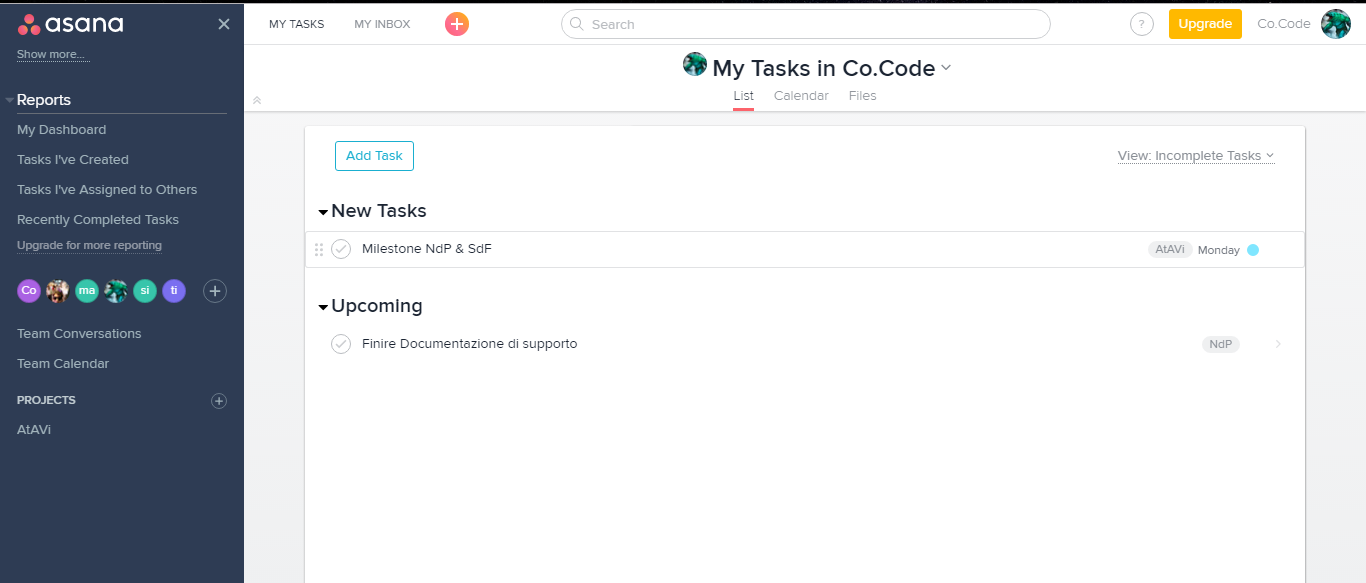
\includegraphics[scale=0.4]{img/asana.png}
\caption{Asana}\label{sec:Figura5}
\end{figure}
 \paragraph{GanttProject} 
 GanttProject è un \gl{software} gratuito per la creazione di grafici rappresentanti l'organizzazione e gestione di compiti e \gl{milestone} all'interno di un \gl{progetto}. Verrà utilizzato nella versione 2.7 o superiore.
\begin{figure}[h]
\centering
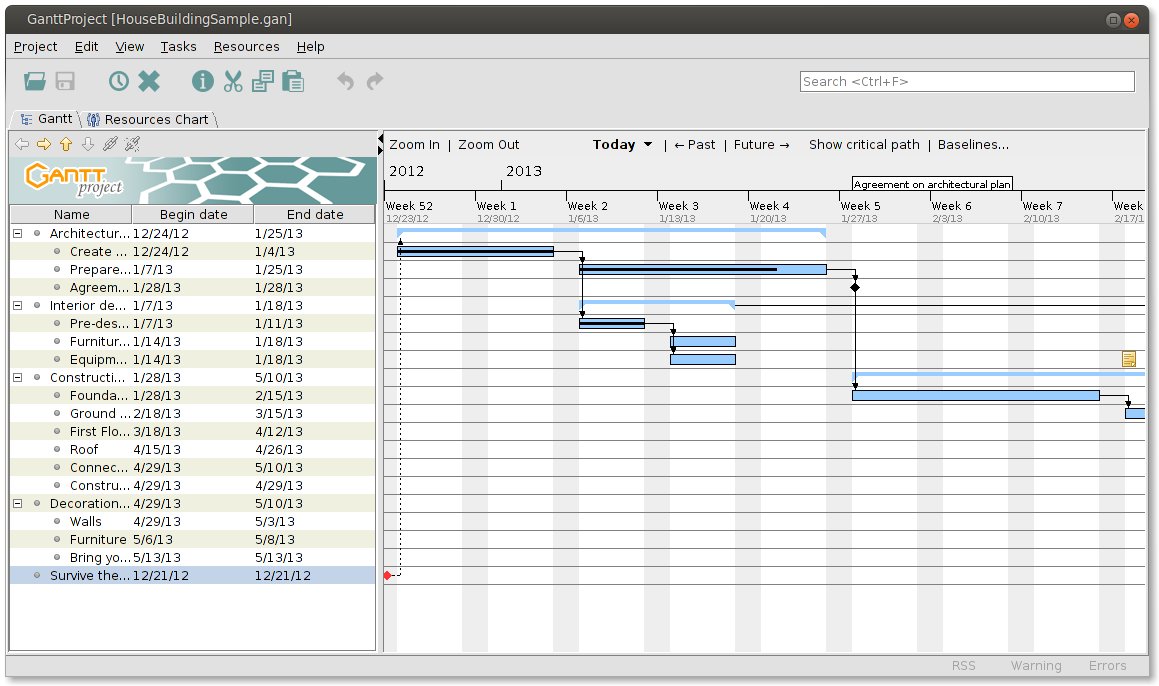
\includegraphics[scale=0.35]{img/gantt.png}
\caption{GanttProject}\label{sec:Figura6}
\end{figure} 
\end{document}
